\documentclass[11pt,a4paper]{article}

\usepackage[T1]{fontenc}
\usepackage[utf8]{inputenc}
\IfFileExists{lmodern.sty}{\usepackage{lmodern}}{\usepackage{mathptmx}}
\usepackage{microtype}
\usepackage[margin=2.5cm]{geometry}
\usepackage{amsmath}
\usepackage{graphicx}
\usepackage{booktabs}
\usepackage{tabularx}
\usepackage{array}
\usepackage{xcolor}
\usepackage{tikz}
\usetikzlibrary{positioning,arrows.meta}
\usepackage[numbers,sort&compress]{natbib}
\usepackage[hidelinks]{hyperref}
\usepackage[capitalise,noabbrev]{cleveref}
\usepackage{authblk}

\definecolor{ecblue}{HTML}{0072B2}
\definecolor{ecgreen}{HTML}{009E73}
\definecolor{ecorange}{HTML}{E69F00}

\newcommand{\ER}{\textsc{EasyResearch}}
\newcommand{\EC}{\textsc{EasyClassifier}}
\newcommand{\EV}{\textsc{EasyVision}}
\newcommand{\pp}{\,pp}
\newcommand{\TBDDOI}{\textcolor{red}{DOI to be added after the v0.1.0 release}}

% generated by benchmarks/easyresearch_honesty_report.py
\newcommand{\RegNData}{9}
\newcommand{\RegRuns}{90}
\newcommand{\RegSeeds}{10}
\newcommand{\RegBiasNaive}{+2.2}
\newcommand{\RegBiasComp}{+2.5}
\newcommand{\RegBiasFinal}{$-$1.0}
\newcommand{\RegMAENaive}{8.2}
\newcommand{\RegMAEComp}{7.9}
\newcommand{\RegMAEFinal}{9.1}
\newcommand{\RegP}{1.3\times10^{-4}}
\newcommand{\RegPds}{0.0098}
\newcommand{\RegCtrlComp}{+11.4}
\newcommand{\RegCtrlFinal}{+6.8}
\newcommand{\RegCtrlCompVal}{$-$0.043}
\newcommand{\RegCtrlFinalVal}{$-$0.089}
\newcommand{\RegCtrlTruthVal}{$-$0.157}
\newcommand{\ScrOut}{0.27}
\newcommand{\ScrIn}{$-$0.33}
\newcommand{\ScrExt}{$-$0.44}
\newcommand{\FcNData}{15}
\newcommand{\FcShufGeo}{19}
\newcommand{\FcShufMedian}{25}
\newcommand{\FcCompGeo}{1}
\newcommand{\FcFinalGeo}{1.5}
\newcommand{\FcShufTyp}{1.48}
\newcommand{\FcCompTyp}{1.28}
\newcommand{\FcFinalTyp}{1.46}
\newcommand{\FcShufBelow}{9}
\newcommand{\FcFinalBelow}{9}
\newcommand{\FcP}{0.1}
\newcommand{\FcToolBetter}{7}
\newcommand{\FcSame}{5}
\newcommand{\FcToolWorse}{3}
\newcommand{\FcTruthGain}{14}
\newcommand{\FcBeatsRule}{12}
\newcommand{\FcBeatsRuleShuf}{10}
\newcommand{\FcRWn}{5}
\newcommand{\FcRWShufML}{5}
\newcommand{\FcRWShufWorse}{5}
\newcommand{\FcRWShufGain}{20}
\newcommand{\FcRWToolNaive}{4}
\newcommand{\SigNData}{4}
\newcommand{\SigRuns}{12}
\newcommand{\SigSeeds}{3}
\newcommand{\SigBiasComp}{0.00}
\newcommand{\SigBiasFinal}{$-$0.02}
\newcommand{\SigMAEComp}{1.9}
\newcommand{\SigMAEFinal}{1.8}
\newcommand{\SigRocketWins}{12}
\newcommand{\SigCtrlComp}{46.9}
\newcommand{\SigCtrlFinal}{42.7}
\newcommand{\SigCtrlTruth}{52.9}


\title{\ER: Honest Regression, Forecasting and Signal Classification\\ for Researchers Who Do Not Program}

\author[1]{Ahmad B. A. Hassanat\thanks{Corresponding author: \href{mailto:ahmad.hassanat@gmail.com}{ahmad.hassanat@gmail.com}}}
\author[2]{Ghada A. Altarawneh\thanks{\href{mailto:ghadaa@mutah.edu.jo}{ghadaa@mutah.edu.jo}}}
\affil[1]{Faculty of Information Technology, Mutah University, Karak, Jordan}
\affil[2]{Department of Accounting, Mutah University, Karak, Jordan}
\date{}

\begin{document}
\maketitle

\begin{abstract}
\EC{} showed that researchers who do not program can obtain honest classification results when the correct evaluation is the default. Most applied studies, however, predict a number, forecast a series or classify recordings, and each task has its own way of producing scores that do not hold on new data. We present \ER, open-source analysis cores for regression, time-series forecasting and signal classification, and \ER{} Desktop, a Windows application that runs these three tasks and \EC's classification without code. All four follow the same rules: everything learned from data is learned on training data only, models keep their published defaults with fixed seeds, the selected model receives a separate final score, forecasts are never evaluated on shuffled data, and every run writes a report with a Methods paragraph and the references for every method used. We measured whether the reported scores are honest by keeping part of each dataset untouched. In regression (\RegNData{} public datasets, \RegRuns{} runs), the common practice overstated $R^2$ by \RegBiasNaive{} points on average and the best comparison score by \RegBiasComp, while \ER's final score was \RegBiasFinal{} (slightly conservative); screening predictors on all rows before cross-validation, which \ER{} does not offer, reported $R^2 = \ScrOut$ on pure noise against \ScrExt{} on new data. In forecasting (\FcNData{} series), shuffled cross-validation over windows of past values promised errors \FcShufGeo\% smaller than its chosen models achieved in the untouched future (geometric mean; median \FcShufMedian\%), while \ER's final-period score was unbiased to within \FcFinalGeo\%; the models \ER{} chose had \FcTruthGain\% lower future error, and on random walks shuffled cross-validation chose a machine-learning model in \FcRWShufML{} of \FcRWn{} series, each worse in the future than repeating the last value, which \ER{} chose \FcRWToolNaive{} times. In signal classification (\SigNData{} UCR datasets) one method won every comparison and neither estimate was biased. The software is available under the MIT license.
\end{abstract}

\noindent\textbf{Keywords:} regression; time-series forecasting; time-series classification; data leakage; nested cross-validation; rolling-origin evaluation; no-code; reproducibility

\begin{table}[h]
\centering\small
\caption{Code metadata.}
\label{tab:metadata}
\begin{tabularx}{\linewidth}{@{}lX@{}}
\toprule
Versions & \ER{} 0.1.0 (analysis cores); \ER{} Desktop 0.3.0; \EC{} 0.8.2 \\
Code repository & \url{https://github.com/ahmadhassant/easyresearch} (desktop application in \texttt{desktop}) \\
Archived version (DOI) & \TBDDOI \\
License & MIT \\
Language and requirements & Python $\geq$ 3.10 with pandas, NumPy, scikit-learn, statsmodels, PyTorch, matplotlib; desktop: C\#/.NET (WPF), Windows x64, bundled Python runtime \\
Documentation & README files of both folders; protocol of the desktop worker (\texttt{desktop/docs/PROTOCOL.md}) \\
Support & GitHub issues; \href{mailto:ahmad.hassanat@gmail.com}{ahmad.hassanat@gmail.com} \\
\bottomrule
\end{tabularx}
\end{table}

%=====================================================================
\section{Motivation and significance}
\label{sec:motivation}

Leakage and optimistic evaluation are among the most common reasons why published machine-learning results fail to replicate \citep{kapoor2023leakage,lones2021pitfalls}. For classification of tabular data we built \EC{} \citep{hassanat2026easyclassifierpaper}, a guided tool that makes the honest procedure the default; on public data from seven fields, the common practice of fitting preprocessing on all rows and reporting the winner's cross-validation score overstated balanced accuracy by 2.9 percentage points on average, against 0.7 for \EC's reported score.

Applied researchers ask other questions as often. A clinician predicts a laboratory value, an economist a wage, an engineer a load; a hydrologist forecasts river flow, a retailer next year's sales; a cardiologist classifies heartbeats, a physiotherapist movement recordings. The same two errors appear in all of them --- learning from the test data before splitting, and reporting the score of the model that won a comparison \citep{varma2006bias,cawley2010overfitting} --- and each task adds its own:
\begin{itemize}
  \item \emph{Regression} invites screening the predictors by their correlation with the outcome on all rows and cross-validating only the final model, the ``wrong way'' to cross-validate \citep{hastie2009esl}.
  \item \emph{Forecasting} has a direction in time. Shuffled cross-validation over windows of past values lets a model learn from values later than those it predicts \citep{tashman2000,bergmeir2012cv}. It can be valid for purely autoregressive models with uncorrelated errors \citep{bergmeir2018note}, but the user of a no-code tool cannot check that condition, and the evaluation of statistical models has no shuffled equivalent at all.
  \item \emph{Signal classification} uses expensive feature extractors and deep networks whose comparison invites reporting the best of several runs.
\end{itemize}

\ER{} extends \EC's answer to these three tasks and puts all four into one desktop application. This paper describes the design (\cref{sec:design}), the three cores (\cref{sec:cores}) and the desktop application (\cref{sec:desktop}), and then measures, on public data with an untouched reference part, whether the scores the software reports are honest (\cref{sec:evaluation}).

%=====================================================================
\section{Design}
\label{sec:design}

The cores share \EC's five principles \citep{hassanat2026easyclassifierpaper}: no code and no jargon unless wanted; honest by default; default parameters without tuning, since tuning adds a further layer of selection and transfers poorly from one small dataset \citep{probst2019tunability}; exact reproducibility with fixed seeds; and output that is ready to report. Two rules are added for the new tasks:

\paragraph{Time is never shuffled.} A series is split once, in time order: a development part and a final period (about the last 20\%). Models are compared at up to five rolling forecast origins in the development part, each model retrained on the values before each origin \citep{tashman2000}; the selected model is then scored in the final period, again retrained before each origin. Only horizons the series can evaluate in this way are offered. An automated test checks that no model's forecast changes when every value after the forecast origin is changed.

\paragraph{Every method is cited.} Each report's Methods paragraph cites every model, distance, evaluation design and measure that was used, and \texttt{citations.txt} lists exactly the report's references with what each is cited for.

\begin{figure}[t]
\centering
\resizebox{\linewidth}{!}{%
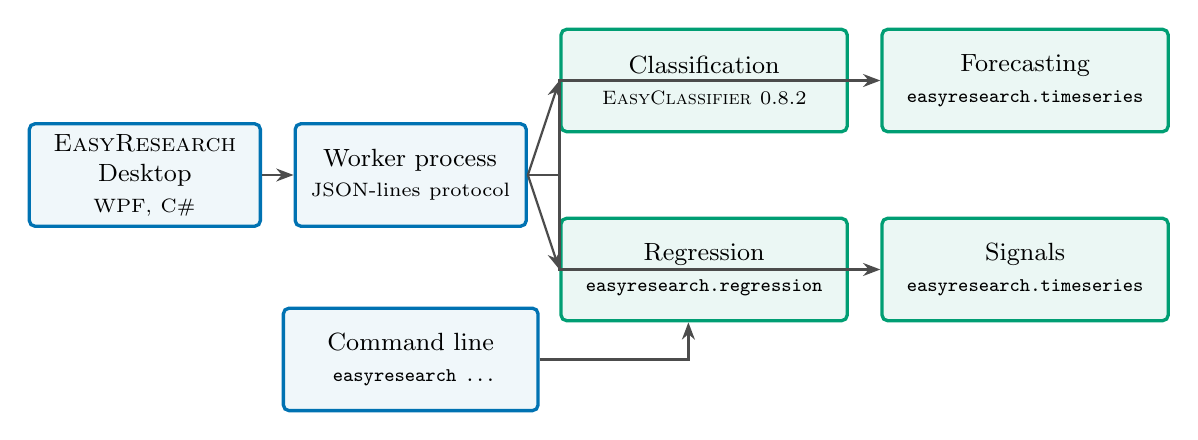
\begin{tikzpicture}[
  node distance=5mm and 4mm,
  box/.style={draw=ecblue, very thick, rounded corners=2pt, fill=ecblue!6,
              align=center, font=\small, text width=27mm, minimum height=13mm},
  core/.style={draw=ecgreen, very thick, rounded corners=2pt, fill=ecgreen!8,
               align=center, font=\small, text width=34mm, minimum height=13mm},
  arr/.style={-{Stealth[length=2.2mm]}, thick, black!70}]
\node[box] (gui) {\ER{} Desktop\\ \scriptsize WPF, C\#};
\node[box, right=of gui] (proto) {Worker process\\ \scriptsize JSON-lines protocol};
\node[core, right=of proto, yshift=12mm] (cls) {Classification\\ \scriptsize \EC{} 0.8.2};
\node[core, right=of proto, yshift=-12mm] (reg) {Regression\\ \scriptsize \texttt{easyresearch.regression}};
\node[core, right=of cls] (fc) {Forecasting\\ \scriptsize \texttt{easyresearch.timeseries}};
\node[core, right=of reg] (sig) {Signals\\ \scriptsize \texttt{easyresearch.timeseries}};
\node[box, below=10mm of proto, text width=30mm] (cli) {Command line\\ \scriptsize \texttt{easyresearch \ldots}};
\draw[arr] (gui) -- (proto);
\draw[arr] (proto.east) -- (cls.west);
\draw[arr] (proto.east) -- (reg.west);
\draw[arr] (proto.east) -- ++(4mm,0) |- (fc.west);
\draw[arr] (proto.east) -- ++(4mm,0) |- (sig.west);
\draw[arr] (cli.east) -| ([xshift=-2mm]reg.south);
\end{tikzpicture}}
\caption{Architecture. The desktop application starts a separate Python worker for every job and talks to it through a versioned JSON-lines protocol; the worker runs the same cores as the command line. Each task is a module with a manifest and an adapter, so a new task (for example computer vision) needs no change to the others.}
\label{fig:architecture}
\end{figure}

%=====================================================================
\section{The analysis cores}
\label{sec:cores}

\subsection{Regression}
Regression reuses \EC's data loading and leakage-free preprocessing \citep{pedregosa2011sklearn}. Ten models are offered: linear and ridge regression, decision tree, random forest \citep{breiman2001rf}, histogram gradient boosting, support vector regression, KNN with the Hassanat distance \citep{hassanat2014arxiv,hassanat2014distance} (columns scaled to 0--1 on training rows; the sign-symmetric form \citep{hassanat2014distance2} for negative values), a neural network, and XGBoost and LightGBM when installed; the fast default set is linear regression, random forest and gradient boosting. SVR and the neural network learn on a standardised target, fitted on training rows, because their defaults assume values of roughly unit size; this is a change of units, not tuning. Models are ranked by $R^2$ on held-out rows, and the selected model receives a final score by nested cross-validation (up to 2{,}000 rows) or on an untouched 20\% test set. Every result is shown next to the reference of always predicting the training mean. Measures are $R^2$, RMSE, MAE, median absolute error, MAPE (only when no actual value is zero or changes sign) and the mean Hassanat similarity percentage, MHSP \citep{hassanat2024mhsp}.

\subsection{Forecasting}
One series with a date column (hourly to yearly; the season length follows) or in row order. Reference rules (naive, seasonal naive) are always included, because a model is useful only if it beats them \citep{hyndman2021fpp3}. Statistical models are exponential smoothing with damped trend and seasonality \citep{hyndman2002ets} and the Theta method \citep{assimakopoulos2000theta}, from statsmodels \citep{seabold2010statsmodels}. Machine-learning models (ridge, random forest, gradient boosting, KNN with the Hassanat distance) predict the next $H$ values at once from the last $L$ values \citep{bontempi2013strategies}, with windows expressed relative to their last value so that tree and neighbour models follow trends. Deep networks (MLP, LSTM, GRU, TCN, N-BEATS, Transformer; PyTorch \citep{paszke2019pytorch}) are optional, because each takes minutes. The model is chosen by MASE \citep{hyndman2006mase} by default; MAE, RMSE, sMAPE and MHSP are reported, with an 80\% band from the comparison errors whose coverage in the final period is checked.

\subsection{Signal classification}
One recording of a single channel per row, from a table or a UCR archive file \citep{dau2019ucr}. Models are KNN with the Hassanat distance, ROCKET with 10{,}000 random convolution kernels \citep{dempster2020rocket}, signal features with a random forest \citep{fulcher2014features}, and optional deep networks (FCN, ResNet, InceptionTime, LSTM). Evaluation is \EC's: stratified cross-validation to compare, ranking by balanced accuracy \citep{brodersen2010balanced}, and nested cross-validation or an untouched stratified 20\% test set for the final score; the most-frequent-class rule is shown for reference.

%=====================================================================
\section{The desktop application}
\label{sec:desktop}

\ER{} Desktop is a portable Windows application that bundles .NET and an isolated Python runtime, so no installation is needed. A sidebar lists the tasks; a fifth, computer vision, appears as a roadmap entry and cannot be selected until its module exists. After a file is read, ``What we noticed'' explains in plain sentences what the analysis will do with it (columns left out and why, empty cells, repeated rows, rare classes, how the final score will be obtained, the length and season of a series). A ``Check and run'' step summarises the analysis and enables Run only when nothing is missing. Advanced options, closed by default, restore \EC's expert choices. Problems such as a damaged file or a file open in another program are explained in one sentence. Every results folder contains the report, tables, predictions or forecasts, figures, the trained model, \texttt{settings.json} (what was asked and what was used), \texttt{versions.txt} (every package version) and a log.

The desktop and the cores are separated by a versioned protocol (\cref{fig:architecture}): each job runs in its own Python process, writes JSON-lines events, and can be cancelled by terminating the process tree. Labels, measures, result tiles and evaluation options come from each module's description of itself, so no screen is specific to one task.

%=====================================================================
\section{Evaluation}
\label{sec:evaluation}

\subsection{Correctness against reference implementations}
Each core was first checked against independent code on public data (\cref{tab:agreement}): the cross-validated $R^2$ of linear regression against a plain scikit-learn pipeline on the same folds, the final-period error of the seasonal naive rule recomputed from the raw series, and \ER's ROCKET against aeon's implementation on the official UCR train/test splits.

\begin{table}[t]
\centering\small
\caption{Agreement with reference implementations (largest absolute difference over the datasets).}
\label{tab:agreement}
\begin{tabular}{@{}llr@{}}
\toprule
Task & Reference & Largest difference \\
\midrule
Regression (5 datasets) & linear-regression $R^2$, scikit-learn pipeline & 0.0000 \\
Forecasting (6 series) & seasonal-naive MAE, recomputed from the series & 0.0000 \\
Signals (4 UCR datasets) & ROCKET accuracy, aeon \texttt{RocketClassifier} & 0.0171 \\
\bottomrule
\end{tabular}
\end{table}

ROCKET draws its kernels at random, so two implementations are not expected to agree exactly; the largest difference was on ArrowHead (80.6\% against 82.3\% accuracy), and the other three datasets agreed exactly.

\subsection{Are the reported scores honest?}

\paragraph{Protocol.} We repeated the design of \EC's honesty benchmark \citep{hassanat2026easyclassifierpaper}. For regression and signals, each dataset was split in half at random (\RegSeeds{} splits for regression, \SigSeeds{} for signals); the first half was analysed with all available standard models (regression) or the default set (signals), and the second half, never touched, gave the true performance of the model each estimate describes, refitted on the whole first half. For forecasting, the first 70\% of each series was the development part and the last 30\% the untouched future, in which the selected model was evaluated at rolling origins one horizon apart, retrained before each origin. The estimates compared with the truth were:
\begin{itemize}
  \item \emph{Common practice}: for regression, preprocessing fitted on all development rows before 5-fold cross-validation and the best model's score reported; for forecasting, the machine-learning models scored by shuffled 5-fold cross-validation over the windows of the development part and the best one reported;
  \item \emph{Comparison best}: the best score in \ER's own leakage-free comparison (selection bias only);
  \item \emph{Final score}: the score \ER{} reports.
\end{itemize}
Controls were a random target (regression; 300 rows, 10 noise predictors), random labels (signals; 200 random-walk recordings) and \FcRWn{} random walks (forecasting), where nothing can be predicted. The benchmark code and all results are in the repository.

\paragraph{Datasets.} Regression: diabetes progression \citep{efron2004lars}, occupational prestige \citep{fox2011car}, New York air quality \citep{chambers1983graphical}, Friedman~\#1 \citep{friedman1991mars}, professors' salaries \citep{fox2011car}, car highway mileage, interlocking directorates \citep{fox2011car}, computer performance, and wages in the Survey of Labour and Income Dynamics \citep{fox2011car}; the last has more than 2{,}000 rows in the development half, so its final score came from an untouched 20\% test set. Forecasting: \FcNData{} monthly, quarterly, yearly and undated series distributed with statsmodels and R, including Mauna Loa CO$_2$, airline passengers \citep{box1976}, UK gas consumption \citep{durbin2001} and Nile flow \citep{cobb1978nile}. Signals: GunPoint, ItalyPowerDemand, ArrowHead and OSULeaf from the UCR archive \citep{dau2019ucr}.

\begin{table}[t]
\centering\small
\caption{Regression: $R^2$ ($\times 100$) estimated on the first half and measured on the untouched second half (mean of 10 random splits). The truth is that of \ER's selected model; the common-practice estimate is compared with its own winner's truth when its bias is computed.}
\label{tab:regression}
\resizebox{\linewidth}{!}{%
\begin{tabular}{@{}lrrrrr@{}}
\toprule
Dataset & Rows & Common practice & Comparison best & \ER{} final & Truth \\
\midrule
Diabetes progression & 221 & 49.4 & 49.2 & 45.9 & 46.6 \\
Occupational prestige (Canada) & 51 & 81.9 & 81.5 & 76.8 & 73.6 \\
New York air quality (ozone) & 58 & 63.9 & 64.9 & 60.4 & 59.5 \\
Friedman \#1 (synthetic, noise sd 1) & 250 & 81.0 & 81.2 & 81.0 & 82.4 \\
Professors' salaries (US) & 196 & 43.0 & 43.6 & 41.0 & 39.8 \\
Car highway mileage (mpg) & 109 & 87.0 & 86.4 & 84.0 & 83.5 \\
Interlocking directorates (Canada) & 124 & 53.4 & 54.9 & 46.7 & 56.4 \\
Computer performance (cpus) & 104 & 86.6 & 87.6 & 80.7 & 83.5 \\
Survey of labour and income (wages) & 2055 & 34.5 & 33.6 & 35.1 & 35.2 \\
\midrule
Random target (control) & 150 & $-$6.1 & $-$4.3 & $-$8.9 & $-$15.7 \\
\bottomrule
\end{tabular}}
\end{table}


\begin{figure}[t]
\centering
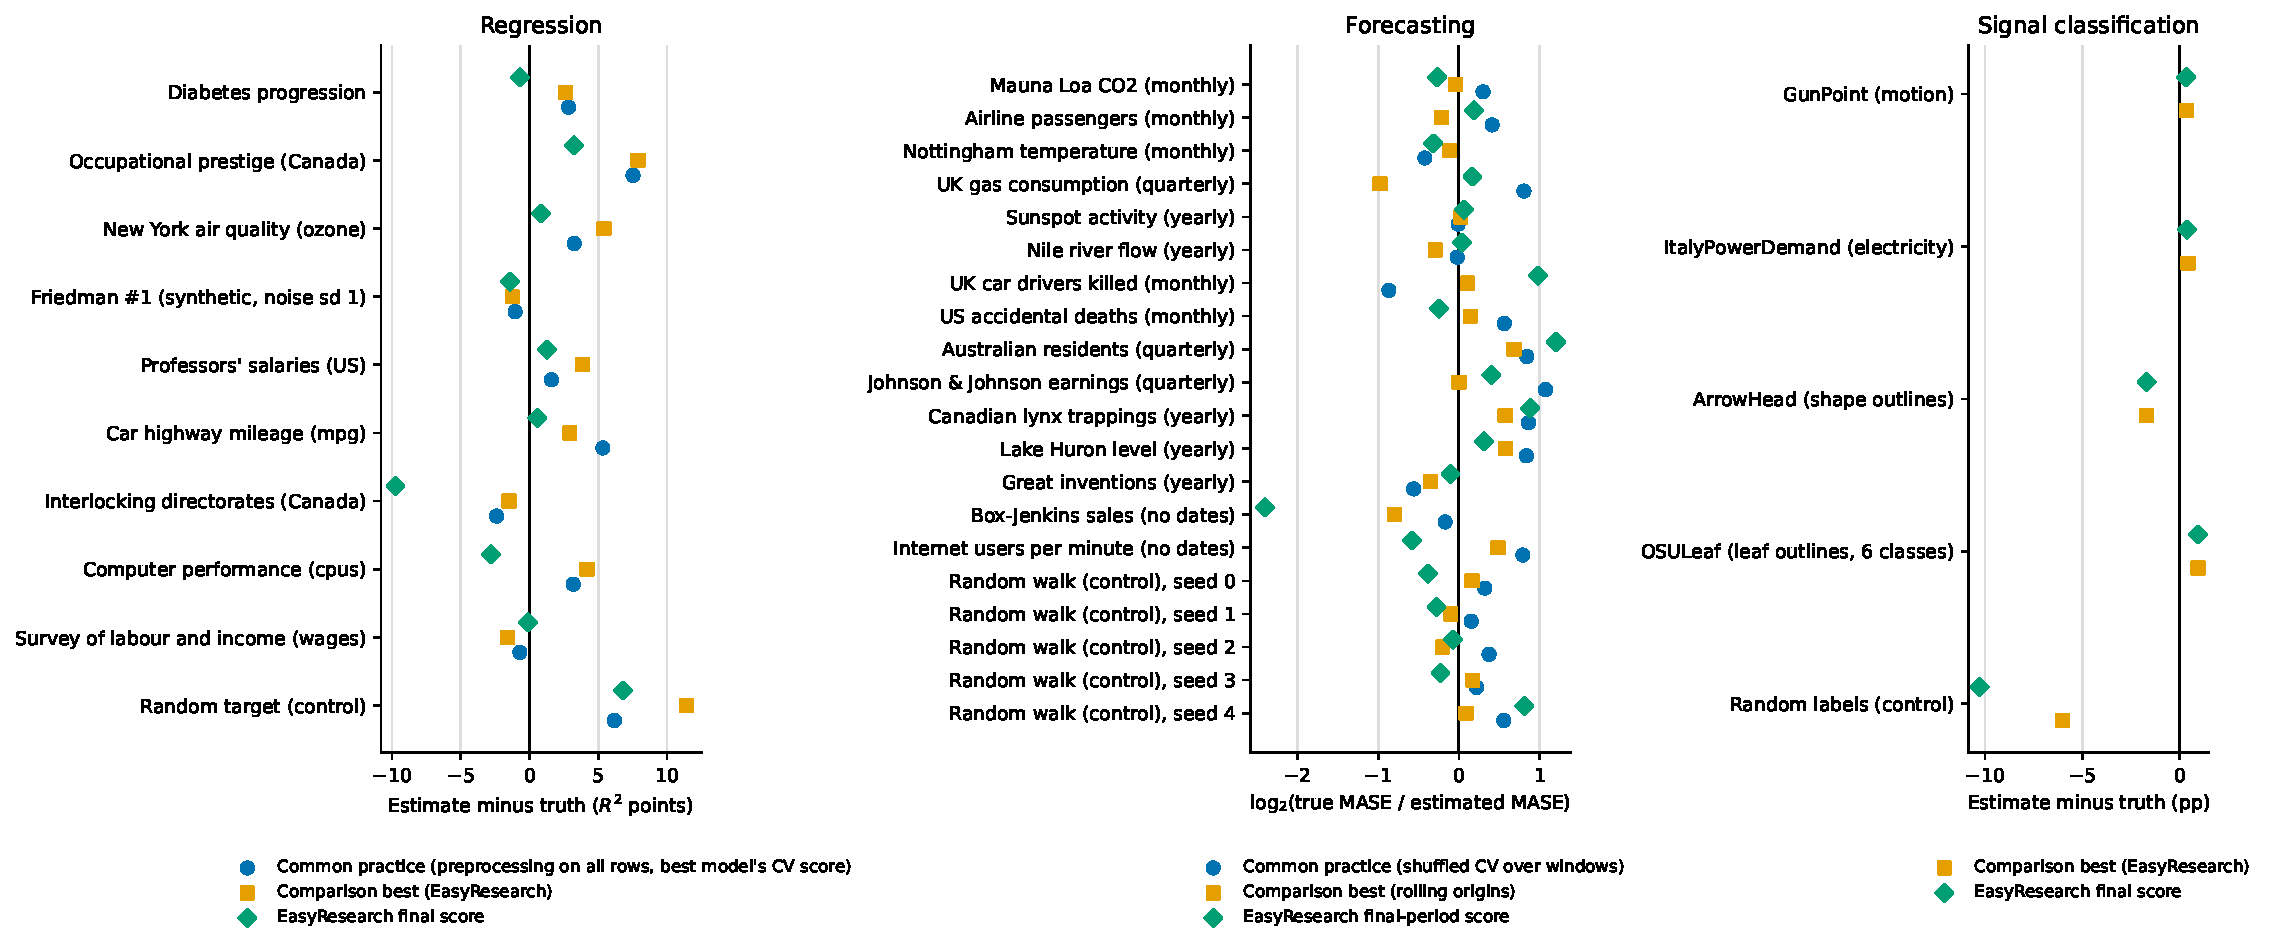
\includegraphics[width=\linewidth]{figures/honesty_easyresearch.pdf}
\caption{Bias of each estimate against the untouched data, per dataset (regression and signals: mean over random splits; forecasting: one development--future split per series). Positive values are optimistic: the estimate promised more than was achieved. Forecasting is shown on the log scale of the ratio of achieved to estimated MASE, so $+1$ means the achieved error was twice the estimate.}
\label{fig:honesty}
\end{figure}

\paragraph{Regression.} \Cref{tab:regression,fig:honesty} show the results. Over the \RegRuns{} runs on real data, the common practice overstated $R^2$ by \RegBiasNaive{} points on average and the best comparison score by \RegBiasComp, while \ER's final score was \RegBiasFinal{} points from the truth, slightly conservative because nested cross-validation trains on fewer rows than the final model (one-sided Wilcoxon signed-rank test that the common practice is more optimistic than the final score: $p = \RegP$; averaging the splits within each dataset first: $p = \RegPds$). On the small halves every estimate was noisy: the mean absolute errors were \RegMAENaive, \RegMAEComp{} and \RegMAEFinal{} points, so the final score removes the optimism but cannot remove the uncertainty of a small sample. Fitting preprocessing on all rows added little on its own (common practice and comparison best were close), as in the classification benchmark; the optimism came from reporting the winner's own score. On the random target, where nothing can be predicted, the best comparison score was $R^2 = \RegCtrlCompVal$, the final score \RegCtrlFinalVal{} and the truth \RegCtrlTruthVal; both reports were negative, which the report states as ``no better than always using the average''.

\paragraph{Screening on all rows.} With 100 rows, 500 noise predictors and a noise outcome, selecting the 10 predictors most correlated with the outcome on all rows and then cross-validating a linear model reported $R^2 = \ScrOut$ on average over \RegSeeds{} draws; repeating the selection inside each fold gave \ScrIn, and the true value on new data was \ScrExt. \ER{} offers no feature selection, partly for this reason.

\begin{table}[t]
\centering\footnotesize
\caption{Forecasting: MASE estimated on the development part (first 70\%) and achieved in the untouched future (last 30\%) by the model each procedure selected; lower is better. $H$ is the horizon. The last column is the naive or seasonal naive rule in the future.}
\label{tab:forecasting}
\resizebox{\linewidth}{!}{%
\begin{tabular}{@{}lrrrrrr@{}}
\toprule
 & & \multicolumn{2}{c}{Shuffled CV} & \multicolumn{2}{c}{\ER} & Rule \\
\cmidrule(lr){3-4}\cmidrule(lr){5-6}
Series & $H$ & estimate (model) & truth & final (model) & truth & truth \\
\midrule
Mauna Loa CO2 (monthly) & 12 & 0.361 (KNN) & 0.444 & 0.447 (Ridge) & 0.371 & 1.204 \\
Airline passengers (monthly) & 10 & 0.396 (Ridge) & 0.527 & 0.462 (Ridge) & 0.527 & 1.275 \\
Nottingham temperature (monthly) & 12 & 0.792 (Ridge) & 0.591 & 0.757 (ETS) & 0.609 & 0.877 \\
UK gas consumption (quarterly) & 4 & 0.927 (Ridge) & 1.622 & 1.443 (Ridge) & 1.622 & 1.740 \\
Sunspot activity (yearly) & 5 & 1.075 (RF) & 1.069 & 1.022 (RF) & 1.069 & 3.432 \\
Nile river flow (yearly) & 5 & 1.008 (RF) & 0.993 & 0.889 (Ridge) & 0.915 & 0.861 \\
UK car drivers killed (monthly) & 12 & 1.100 (RF) & 0.603 & 0.458 (ETS) & 0.904 & 1.216 \\
US accidental deaths (monthly) & 5 & 1.169 (RF) & 1.729 & 0.607 (seas.\ naive) & 0.512 & 0.512 \\
Australian residents (quarterly) & 4 & 0.072 (Ridge) & 0.129 & 0.052 (ETS) & 0.121 & 1.211 \\
Johnson \& Johnson earnings (quarterly) & 4 & 0.587 (Ridge) & 1.237 & 0.994 (ETS) & 1.314 & 2.627 \\
Canadian lynx trappings (yearly) & 8 & 0.891 (RF) & 1.623 & 0.879 (RF) & 1.623 & 2.759 \\
Lake Huron level (yearly) & 6 & 1.451 (RF) & 2.593 & 2.086 (RF) & 2.593 & 2.243 \\
Great inventions (yearly) & 7 & 0.999 (RF) & 0.678 & 0.708 (Theta) & 0.659 & 0.912 \\
Box-Jenkins sales (no dates) & 10 & 3.428 (KNN) & 3.048 & 7.350 (ETS) & 1.387 & 1.851 \\
Internet users per minute (no dates) & 7 & 2.969 (RF) & 5.149 & 5.057 (ETS) & 3.381 & 4.819 \\
\midrule
Random walk (control), seed 0 & 10 & 1.879 (KNN) & 2.349 & 2.378 (naive) & 1.823 & 1.823 \\
Random walk (control), seed 1 & 10 & 2.280 (KNN) & 2.536 & 2.574 (naive) & 2.125 & 2.125 \\
Random walk (control), seed 2 & 10 & 1.983 (RF) & 2.572 & 2.654 (naive) & 2.527 & 2.527 \\
Random walk (control), seed 3 & 10 & 2.306 (RF) & 2.686 & 2.742 (naive) & 2.341 & 2.341 \\
Random walk (control), seed 4 & 10 & 2.150 (RF) & 3.162 & 1.543 (ETS) & 2.711 & 2.650 \\
\bottomrule
\end{tabular}}
\end{table}


\paragraph{Forecasting.} \Cref{tab:forecasting} shows the results as MASE. Because relative errors are asymmetric, we summarise the ratio of estimated to achieved MASE on the log scale. Shuffled cross-validation promised a smaller error than its selected model achieved in the future on \FcShufBelow{} of \FcNData{} series; on average (geometric mean) the promised error was \FcShufGeo\% too small (median \FcShufMedian\%). \ER's final-period score was unbiased on average (geometric mean within \FcFinalGeo\% of the truth) but, measured on a short final period, it was as variable as the shuffled estimate: a typical estimate was off by a factor of \FcFinalTyp{} (shuffled \FcShufTyp, comparison best \FcCompTyp), and the difference in bias was not significant over \FcNData{} series ($p = \FcP$). The choice of model mattered more than the estimate: the models \ER{} selected by rolling-origin comparison had a lower future error than those selected by shuffled cross-validation on \FcToolBetter{} series, the same model on \FcSame{} and a higher error on \FcToolWorse{} (\FcTruthGain\% lower on average), and they beat the naive or seasonal naive rule in the future on \FcBeatsRule{} series against \FcBeatsRuleShuf. On the random walks, shuffled cross-validation selected a machine-learning model in \FcRWShufML{} of \FcRWn{} series and promised an error \FcRWShufGain\% below what it achieved; \FcRWShufWorse{} of these models were worse in the future than repeating the last value. \ER{} selected the naive rule itself on \FcRWToolNaive{} of the \FcRWn{} random walks.

\begin{table}[t]
\centering\small
\caption{Signal classification: balanced accuracy (\%) estimated on the first half and measured on the untouched second half (mean of 3 random stratified splits), default model set.}
\label{tab:signals}
\begin{tabular}{@{}lrrrr@{}}
\toprule
Dataset & Recordings & Comparison best & \ER{} final & Truth \\
\midrule
GunPoint (motion) & 100 & 100.0 & 100.0 & 99.7 \\
ItalyPowerDemand (electricity) & 548 & 97.4 & 97.4 & 97.0 \\
ArrowHead (shape outlines) & 105 & 93.4 & 93.4 & 95.1 \\
OSULeaf (leaf outlines, 6 classes) & 221 & 94.0 & 94.0 & 93.0 \\
\midrule
Random labels (control) & 100 & 46.9 & 42.7 & 52.9 \\
\bottomrule
\end{tabular}
\end{table}


\paragraph{Signals.} \Cref{tab:signals} shows the results. ROCKET won the comparison in all \SigRuns{} runs on real data, so there was no selection to correct: the best comparison score and the final score were both unbiased on average (\SigBiasComp{} and \SigBiasFinal{} points; mean absolute errors \SigMAEComp{} and \SigMAEFinal). On random labels the comparison best reported \SigCtrlComp\% balanced accuracy, the final score \SigCtrlFinal\% and the truth on the untouched half was \SigCtrlTruth\%; all three are chance level within the noise of 100 recordings. The final score therefore costs computing time without changing the result when one method clearly dominates, and protects the user when it does not; the software cannot know in advance which case applies.

%=====================================================================
\section{Impact, limitations and future work}
\label{sec:impact}

\paragraph{Impact.} \ER{} brings honest regression, forecasting and signal classification to researchers who do not program, in the same application as \EC's classification, with plain-language explanations and reports that a reviewer can check. The benchmark shows where the protection matters. Shuffled evaluation of forecasts promised errors about a fifth smaller than were achieved and, on series where nothing can be forecast, preferred machine-learning models that lost to the simplest rule; in regression, reporting the winner's comparison score was optimistic. Where one method clearly dominates, as ROCKET did on the signal datasets, the honest final score changes little. In every task, estimates from small samples remained noisy, which a tool can report but not remove.

\paragraph{Limitations.} Signal classification handles one channel per recording; several channels and long recordings cut into windows are planned. Forecasting handles one series without explanatory variables. Several rows per subject (repeated measurements) are not yet grouped in cross-validation, so users with such data must aggregate first. The desktop application runs on Windows only. Deep models are slow on a normal computer and are therefore optional. The benchmark used modest datasets, a single development--future split per series for forecasting and three splits per dataset for signals; it shows the direction and order of the biases, not their exact size elsewhere.

\paragraph{Future work.} Computer vision (\EV) is the next module, with subject-wise splitting, augmentation confined to training images and a mandatory check for copied images; grouped cross-validation, multichannel signals and a server version follow.

%=====================================================================
\section{Conclusions}
\ER{} extends the rules of \EC{} to regression, forecasting and signal classification and brings all four tasks into one application for researchers who do not program. Its reported scores were free of the optimism of the common practice in regression and forecasting, unbiased where there was nothing to correct, and on data where nothing can be predicted it said so.

\section*{Acknowledgements}
The authors thank the developers of scikit-learn, statsmodels, PyTorch, aeon, pandas, NumPy and matplotlib, and the authors of the public datasets used in the evaluation. Parts of the software, the benchmark scripts and this manuscript were prepared with the help of Claude (Anthropic), an AI assistant, which was used for coding support, drafting and editing. The authors designed the software and the study, checked all code, results and text, and take full responsibility for the content of this paper.

\section*{Software and data availability}
{\sloppy
\begin{itemize}
  \item Source code of \ER{} and \ER{} Desktop: \url{https://github.com/ahmadhassant/easyresearch}; archived at Zenodo, \TBDDOI.
  \item \EC: \url{https://github.com/ahmadhassant/easyclassifier}; Zenodo, \href{https://doi.org/10.5281/zenodo.23122901}{doi:10.5281/zenodo.23122901} (all versions).
  \item Benchmarks: \nolinkurl{benchmarks/easyresearch_benchmarks.py} and \nolinkurl{benchmarks/easyresearch_honesty.py} in the same repository, with all results; every dataset is installed with pip.
\end{itemize}}

\bibliographystyle{plainnat}
\bibliography{references}

\end{document}
